Según la Fundación de la Universidad Autónoma de Madrid, la comunicación es el proceso mediante el cual transmitimos y recibimos datos, ideas, opiniones y actitudes para lograr comprensión y acción. Este concepto es importante ya que nos ayuda a entender de forma básica en qué consiste este proceso y cómo es posible implementarlo de forma activa para crear una interacción más orgánica entre el usuario y el animatrónico, pues el objetivo es generar cierta semejanza con la interacción humana.

A partir de este objetivo, surge la idea de implementar un chatbot para crear esa fluidez y amplitud de conversación entre el animatrónico y el usuario para alcanzar una comunicación adecuada. Un chatbot es una pieza de software con inteligencia artificial en un dispositivo, aplicación, sitio web u otras redes que intentan medir las necesidades de los consumidores y luego ayudarlos a realizar una tarea particular. En general, existen dos variantes de chatbots: basado en reglas y auto aprendizaje. El primero responde preguntas basadas en algunas reglas que previamente han sido entrenadas. Manejan consultas simples pero fallan en las complejas. Los de auto aprendizaje utilizan técnicas de aprendizaje automático y son mucho más eficientes; existen de dos tipos: basados en recuperación y generativos.

En los modelos basados en recuperación, estos bots utilizan cierta heurística para seleccionar de una base de datos una respuesta, esto hace que tengan un conocimiento limitado y controlable y utiliza el mensaje y el contexto de la conversación para seleccionar la respuesta idónea.

En los modelos generativos, el bot es capaz de tomar palabra por palabra y generar una respuesta que no siempre viene del conjunto de datos previos. Esto los hace más inteligentes y con una capacidad amplia de aprendizaje.

Teniendo en cuenta estas opciones, es claro que para cumplir el objetivo del proyecto es necesario un chatbot con un modelo basado en recuperación, pues es importante que la interacción se sienta orgánica para el usuario (pues vemos que este modelo no se limita tanto como el basado en reglas) pero no se necesita que el bot recopile más datos de la conversación para generar respuestas específicas, pues es importante limitar la información y formulación de respuestas del bot para evitar inconvenientes que se puedan generar por conversaciones pasadas.


\begin{figure}[t]
    \centering
    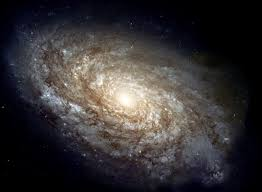
\includegraphics[width=0.5\textwidth]{galaxia.jpg}
    \caption{Una imagen de una galaxia.}
    \label{fig:mesh1}
\end{figure}

Donec a libero vel lacus tincidunt dapibus. Nullam et leo volutpat dui feugiat volutpat vel lacinia ante. Donec finibus risus at facilisis gravida. Cras efficitur felis elementum purus finibus ultricies. Nunc sit amet diam egestas, blandit mauris nec, gravida nisi. In a arcu eu nunc mattis dictum sed placerat arcu. Morbi sit amet venenatis lectus, vitae lobortis nisl. Pellentesque id mattis magna, et convallis leo. Maecenas ultricies hendrerit quam vel ornare. Pellentesque fermentum aliquet velit quis malesuada. Proin commodo, est ultrices rhoncus scelerisque, massa nulla congue tellus, ut porta ante ante vitae nisl. In pharetra quam et urna dictum scelerisque. Aliquam in metus velit. Phasellus aliquet velit molestie, tincidunt purus vestibulum, aliquet odio. Sed augue odio, scelerisque non mi et, pulvinar bibendum justo. Vestibulum sed hendrerit urna.

Donec a lacus quis mi volutpat mollis ac ut lorem. Nulla porta venenatis faucibus. Fusce metus lectus, ullamcorper vel risus laoreet, consequat faucibus sapien. Donec vitae ultrices mauris, dignissim sodales eros. Integer hendrerit elementum ipsum a vestibulum. Vivamus in pretium orci. Fusce condimentum, nibh tempor sagittis laoreet, dui erat luctus neque, a ultrices arcu mauris eget massa. Duis quis ante metus. Interdum et malesuada fames ac ante ipsum primis in faucibus.

\begin{table}[b]
\centering
\begin{tabular}{|c|c|c|c|}
\hline
\textbf{item} & \textbf{característica 1} & \textbf{característica 2} & \textbf{característica 3} \\ \hline
1             & 3234                      & 12323                     & 4343                      \\ \hline
2             & 1332                      & 123123                    & 12                        \\ \hline
3             & 1232                      & 4334                      & 12312                     \\ \hline
\end{tabular}
\caption{Tabla generada automáticamente.}
    \label{cuadro:prueba2}
\end{table}

Según la investigación realizada en \cite{lee2001biomedical}, vestibulum laoreet tortor enim, nec tristique turpis dapibus id. Nam quis erat ac nibh imperdiet placerat et a sapien. Aliquam sollicitudin, leo a aliquam vestibulum, lectus eros maximus justo, eu tincidunt justo ipsum non risus. Curabitur ultrices mi vitae elit venenatis, vel semper orci consequat. Nulla ac mauris vitae orci tincidunt mattis. Mauris risus justo, luctus non diam in, dapibus scelerisque eros. Donec fringilla risus sit amet sapien tempus viverra. Quisque quis justo ut enim gravida mollis in vulputate libero. Maecenas auctor accumsan turpis, id dapibus odio aliquet sit amet. Sed feugiat libero eget facilisis finibus. Sed vitae nulla nec felis porta convallis a in purus. Integer finibus efficitur lorem at aliquet. Etiam venenatis velit non tempus porttitor.

\subsection*{Primer tema}

Suspendisse tincidunt a orci sed vehicula. Aenean ac mauris enim. Duis vitae fringilla augue. Mauris fringilla neque ac nunc aliquet porta. Praesent quis elit convallis, vehicula leo a, tincidunt leo. Curabitur vitae ligula non leo faucibus cursus sit amet nec ex. Proin mollis lectus in odio aliquet, eu tristique lacus aliquet. Aliquam auctor eget lorem quis porttitor. Duis sagittis eros ac diam ornare, id auctor elit cursus. Morbi vel dolor et odio laoreet ornare. Cras sit amet pretium neque. Mauris vestibulum ante sit amet eros rutrum eleifend ac a sapien. Nullam vitae convallis eros. Proin blandit a nulla nec hendrerit. Fusce ultrices, nibh in mattis consequat, nisi libero rutrum lacus, vitae vulputate lorem tellus vitae enim.

\subsubsection*{Primer subtema}

Quisque feugiat felis diam. Maecenas elementum, neque ut ornare tristique, nulla sem semper diam, vel imperdiet purus arcu sit amet magna. Nullam tempus eleifend ultrices. Maecenas pharetra ac leo eget mattis. Donec suscipit arcu justo, ac finibus diam scelerisque sit amet. Nulla et porta urna. Donec vel ultrices lectus. Quisque id molestie tellus. Vivamus vitae elit sit amet ipsum tincidunt sodales eget eget tortor. Quisque vitae placerat ipsum. Donec malesuada ipsum a consectetur venenatis.
